% $Id$

One of the most interesting problems in astrophysics is that of \emph{dark
matter}. Dark matter is so called because it has eluded detection through its
emission or absorbsion of electomagnetic radiation. Our knowlege of its
existance comes from the gravitational interaction of dark matter with
luminous matter in the universe. There have been several ideas proposed to
explain the nature of dark matter, chief among these are \emph{weakly
interacting massive particles} (WIMPs) and \emph{massive astrophysical
compact halo objects} (MACHOs)\cite{Griest:1990vu}.  WIMPs, supersymmertic
particles produced as a relic of the big bang, are outside the scope of this
thesis\footnote{We refer to \cite{Griest:1995gs} for a review of the nature of
dark matter.}. In this chapter, we review the evidence for dark matter in the
form of MACHOs in the Galactic halo. The nature of MACHOs is unknown; we
review a proposal that suggests that if MACHOs are primordial black holes
(PBHs) formed in the early universe, then some of the PBHMACHOs may be in
binary systems\cite{Nakamura:1997sm}. The detection of gravitational waves
from the inspiral and coalescence of these binary black hole machos
(BBHMACHOs) is the motivation for this thesis.

\section{Dark Matter In The Galactic Halo}
\label{s:darkmatter}

Dark matter is detected by its gravitational interaction with luminous matter.
Strong evidence for the presence of dark matter in the universe comes from the
study of galactic rotation curves; measurements of the velocities of luminous
matter in the disks of spiral galaxies as a function of galactic radius.  Let
us consider a simple rotational model for the disk of a spiral galaxy.
Consider a star with mass $m_s$ orbiting at radius $r$ in the outer part of
the galaxy's disk. Newtonian dynanics tells us that if the mass inside radius
$r$ is $m_g$ then
\begin{equation}
\frac{Gm_g m_s}{r^2} = \frac{m_s v_s^2}{r}
\label{eq:newtongalaxy}
\end{equation}
where $v_s$ is the velocity of the star and $G$ is the gravitational constant. 
If we assume that as we increse $r$, the change in the $m_g$ is negligable.
This is a reasonable assumption towards the edge of the disk, since the mass
is concentrated towards the center of the galaxy.  We can see from equation
\ref{eq:newtongalaxy} that we would expect that the velocity of stars at the
edge of the galactic disk would fall off as 
\begin{equation}
v_s \propto \frac{1}{\sqrt{r}}
\end{equation}
and so a typical galactic rotation curve would fall off as $r^{-1/2}$.
Galactic rotation curves, measuring using the doppler shift of the
$21$~cm hydrogen line, have been measured for several galaxies. It is found
that the rotation curves to not fall off as expected. Instead they are flat
out to the edge of the visible matter in the disk, as shown in
figure~\ref{f:rotcurves}.  This surprising result suggests that most of the
matter in galaxies does not emit light but is gravitationally coupled to the
visible matter. Rotation curves suggest that around 80\%--90\% of the matter
in spiral galaxies is in the form of dark matter\cite{Sancisi:1987}.

Since we have been unable to observe the dark matter component of the galaxy,
we must infer its distribution and density from the indirect obesrvations and
numerical simulations of galaxy formation. Consider the evolution of a spatial
distribution of baryonic matter. Baryonic matter is the typical luminous
matter that we see composed of neutrons, protons, electrons and other baryons.
If the distribution is initially spherical and rotating with some angular
momentum, $L$, then over time the matter will lose energy through inelastic
collisions. Since the angular momentum of the system must be conserved,
howeverm the initial distribution will collapse to a rotating disk.  This toy
model is typical of the formation of galaxtic disks from baryonic matter. On
the other hand, if the initially spherical distribution is composed of dark
matter, the only collisions that the population will undergo are elastic,
because the dark matter is weakly interacting. As a result of this, if the
dark matter is initially distributed uniformly with and isotropic, it will
maintain this distribution as it evolves.

We may guess that the dark matter halos are at least as old os the visible
matter as they are much more massive. Since the dark matter is gravitationally
bound to the visible matter in the disk, it is reasonable to assume that the
visible disk and dark halo are in thermal equilibrium with some characteristic
mean square velocity. Since we do not expect a spherical dark matter halo to
collapse to a disk, the simplest possible assumption is that the dark halo is
a spherical, isothermal distribution of dark matter. We may ask what the
dark matter density is in the neighbourhood of the earth. If we assume that
the density of the dark matter is $\rho(r)$ then for a spherical halo the mass
within a thin shell of width $dr$ is
\begin{equation}
dM(r) = 4\pi r^2 \rho(r)\, dr.
\label{eq:simplehalodensity}
\end{equation}
Using Newtonian dynamics, the velocity, $v$, of a particle of mass $m$ at
radius $r$ is
\begin{equation}
\begin{split}
\frac{GM(r)m}{r^2} &= \frac{mv^2}{r} \\
v^2 &= \frac{GM(r)}{r}.
\end{split}
\end{equation}
The galactic rotation curves tell us that the velocity is independent of the
radius, so
\begin{equation}
M(r) = \frac{v^2r}{G}.
\end{equation}
Differentiating this with respect to $r$ and substituting the result into
equation \ref{eq:simplehalodensity}, we obtain
\begin{equation}
\frac{dM(r)}{dr} = \frac{v^2}{G} = 4\pi r^2\rho(r)
\end{equation}
which gives
\begin{equation}
\rho(r) = \frac{v^2}{4\pi r^2 G}.
\label{eq:simplehalodensity2}
\end{equation}
Since the dark and visible matter are in thermal equilibrium, we may use the
measrued rotational velocity of local stars about the galactic center as the
velocity of the dark matter. The earth is approximately $8$~kPc from the
galactic center and the rotational velocity of objects at this radius is
$v\sim 200\mathrm{km\,s}^-1$. Using these values in equation
(\ref{eq:simplehalodensity2}), we obtain a value of
\begin{equation}
\rho(r_E) = 7.6 \times 10^{-25}\, \mathrm{g}\,\mathrm{cm}^{-3}.
\end{equation}
Clearly equation (\ref{eq:simplehalodensity2}) cannot be true at all radii, as
it suggests that $\rho \rightarrow \infty$ as $r \rightarrow \infty$. It is
observered that rotation velocities fall to zero as $r\rightarrow 0$. The data
at small $r$ is consistent with the dark matter having a constant \emph{core
density}, $\rho_c$ within a \emph{core radius}, $a$. The halo density then
becomes
\begin{equation}
\rho(r) = \frac{\rho_c}{1 + \left(\frac{r}{a}\right)^2}.
\label{eq:simplehalodensity3}
\end{equation}.
The values of $\rho_c$ and $a$ are obtained from fitting measured galactic
rotation curves to equation (\ref{eq:simplehalodensity3}) using data near the
galactic center. 

There is, in fact, no evidence to suggest that halos are
exactly spherical; the halo density may be flattened\cite{Rix:1996}. For a
flattened halo the dark matter density becomes
\begin{equation}
\rho(R,z) = \frac{\rho_c r^2_c}{a^2 + R^2 + z^2/q^2}
\label{eq:simplehalodensity4}
\end{equation}
where $R$ and $z$ are galactocentric cylindrical coordinates and $q$ is a
parameter that describes the flattening of the halo. Careful modelling of the
Galaxy\cite{1995ApJ...449L.123G}, suggests that the local halo density is
\begin{equation}
\rho_(r_E) = 9.2_{-3.1}^{+3.8} \times 10^{-25}\, \mathrm{g}\,\mathrm{cm}^{-3}
\end{equation}
or approximately $0.01\,M_\odot.\,\mathrm{pc}^{-3}$.

\section{MACHOs in the Galactic Halo}
\label{s:machos}

Galactic rotation curves provide strong evidence that spiral galaxies such
as the Milky Way are surrrounded by a large quantity of dark matter. They
tell us nothing about the nature of this dark matter, however, other than that
it interacts gravitationally with the luminous matter. A wide variety of
candiates have been proposed to explain the nature of dark matter. These
generally fall into two classes. The first class consists of elementary
particles such as axions\cite{Weinberg:1977ma} or weakly interacting massive
particles (WIMPs)\cite{Goodman:1984dc}. Axions are particles proposed to
explain the lack of CP violation in the strong interaction and WIMPs are
supersymmetric particles, such as the neutralio. Such dark matter candidates
are outside the scope of this thesis. Active searches for WIMPs and axions are
underway and we refer to \cite{Griest:1995gs} for a review of the particle
physics dark matter candidates.  Here we are concerned with the second class
of dark matter candidates known as \emph{massive astrophysical compact halo
objects} or MACHOs.  MACHOs are objects such as brown dwarfs (stars with
insufficient mass to burn hydrogen), red dwarfs (stars with just enough mass
to induce nuclear fusion), white dwarfs (remnnants of $1$--$8\,M_\odot$ stars)
or black holes located in the halos of galaxies.  Optical and infrared
observations in the early 1990's were not sensitive enough to contrain the
fraction of the halo in MACHOs\cite{1994MNRAS.266..775K} and the method of
\emph{gravitational lensing} was suggested\cite{Paczynski:1985jf} as a method
for detecting halo dark matter in the form of MACHOs.

\subsection{Gravitational Lensing of Light}
\label{ss:microlensing}

Gravitational lensing is caused by the bending of light around a massive
object. Let us assume that a MACHO produces a spherically symmetric
gravitational field; the geometry of space-time around the MACHO satisfies the
Schwarzchild solution. Recall that the orbits of Schwazchild space-time
satisfy
\begin{equation}
\frac{d^2 u}{d\phi^2} + u = \epsilon \frac{GM}{l^2} + 3GMu^2
\label{eq:schorbit}
\end{equation}
where $u = r^{-1}$, $l$ is a constant (of angular momentum), $M$ is the mass
of the MACHO and $\epsilon = -1,0$ or $+1$ for spaceline, null or timeline
trajectories respectively. Consider the scattering of light by a MACHO. Denote
by $b$ the \emph{impact parameter} of the light, that is the minimum distance
of the photon to the MACHO, as shown in figure \ref{f:scattering}. For a
photon $\epsilon = 0$ and so equation (\ref{eq:schorbit}) becomes
\begin{equation}
\frac{d^2 u}{d\phi^2} + u =  3GMu^2.
\label{eq:schphotonorbit}
\end{equation}
If $R$ is the radius of the MACHO, then
\begin{equation}
\frac{3GMu^2}{u} = \frac{3GM}{R} \frac{R}{r}.
\end{equation}
Therefore if $b \gg R$ then $3GMu^2 \ll u$ and we may treat the term
$3GMu^2$ as a perturbation. Let us write
\begin{equation}
u = u_0 + u_1 + \cdots
\end{equation}
and so equation (\ref{eq:schphotonorbit}) becomes
\begin{equation}
u_0'' + u_1'' + \cdots + u_0 + u_1 + \cdots = 3GM\left(u_0 + u_1 +
\cdots\right)^2 + 3GMu_0^2 + \cdots
\end{equation}
where prime denotes differentiation with respect to $\phi$. $u_0$ satisfies
\begin{equation}
u_0'' + u_0 = 0
\end{equation}
which has solution
\begin{equation}
u_0 = A \sin \left(\phi - \phi_0\right)
\end{equation}
where $A$ and $\phi_0$ are constants. We are free to choose any value for
$\phi_0$ as it simply choses an orientation for the axes in figure
\ref{f:scattering}, so let $\phi_0 = \pi /2$. The value $\phi = \pi / 2$
gives the distance of closed approach which fixes $A = b^{-1}$. Now $u_1$
satisfies
\begin{equation}
\begin{split}
u_1'' + u_1 &= \frac{3GM}{b^2} \sin^2 \phi \\
&= \frac{3GM}{2b^2}\left(1 - \cos 2\phi\right).
\label{eq:u1eq}
\end{split}
\end{equation}
Inspection suggests a solution of the form
\begin{equation}
u_1 = \frac{3GM}{2b^2} + \alpha \cos 2\phi.
\end{equation}
Substituting this into equation (\ref{eq:u1eq}) we find that
\begin{equation}
-4\alpha \cos 2\phi + \frac{3GM}{2b^2} + \alpha\cos 2\phi =
\frac{3GM}{2b^2} - \alpha\cos 2\phi
\end{equation}
and so $\alpha = GM/2b^2$. The solution for $u$, up to first order, is
therefore
\begin{equation}
u = \frac{1}{b} \sin \phi + \frac{GM}{2b^2}\left(3 + \cos 2\phi\right).
\end{equation}
As $r \rightarrow \infty$, $u \rightarrow 0$ and $\phi \rightarrow - \delta/2$,
so
\begin{equation}
0 = \frac{1}{b} \sin \left(-\frac{\delta}{2}\right) + 
\frac{GM}{2b^2} \left(3 + \cos(-\delta)\right)
\end{equation}
For small $\delta$, $\sin(-\delta/2) \approx -\delta/2$ and $\cos(-\delta)
\approx 1$, so
\begin{align}
0 &\approx - \frac{\delta}{2b} + \frac{2GM}{b^2} \\
\delta &\approx \frac{4GM}{b}
\end{align}
The total deflection of the light is
\begin{equation}
\delta = \frac{4GM}{c^2 b}.
\end{equation}
Suppose a MACHO lens is at a distance $D_\mathrm{SL}$ from a source star and
an observer is at a distance $D_\mathrm{L}$ from the MACHO as shown in figure
\ref{f:macholens}. The then the ray of light from the source that encounters
the MACHO with critical impact parameter $r_\mathrm{E}$ will reach the
observer. Simple geometry shows that
\begin{equation}
\delta = \theta_\mathrm{S} + \theta_\mathrm{O} =
\frac{r_\mathrm{E}}{D_\mathrm{L}} + \frac{r_\mathrm{E}}{D_\mathrm{SL}} =
\frac{4GM}{c^2r_\mathrm{E}}
\end{equation}
therefore the observer sees the lens light when the ray is at the
\emph{Einstein radius}, $r_\mathrm{E}$, given by
\begin{equation}
r_\mathrm{E} = \sqrt{\frac{4GM}{c^2} \frac{D_\mathrm{SL} D_\mathrm{L}}
{D_\mathrm{SL} + D_\mathrm{L}}}.
\end{equation}
If the source, MACHO and observer are co-linear, as shown in figure
\ref{f:macholens}, then the observer sees a bright ring of radius
$r_\mathrm{E}$ around the MACHO. The angular radius of this ring is the
\emph{Einstein angle},
\begin{equation}
\theta_\mathrm{E} = \sqrt{\frac{4GM}{c^2} \frac{D_\mathrm{SL}}
{D_\mathrm{L}\left(D_\mathrm{SL} + D_\mathrm{L}\right)}}.
\end{equation}
In the realistic case of slight misaligment, then the lensed star will appear
as two small arcs. Consider a MACHO of mass $0.5\,M_\odot$ at a distance of $D
= 25$~kpc lensing a star in the Large Magellanic Cloud (LMC) at a distance of
$50$~kpc. Then
\begin{equation}
\theta_\mathrm{E} = \sqrt{\frac{2GM}{Dc^2}} \approx 10^{-10} \approx 2 \times
10^{-5}"
\end{equation}
which is far too small to be resolved, however the lensing produces an
apparent amplification of the source star\cite{1964MNRAS.128..295R} by a
factor of
\begin{equation}
A = \frac{u^2 + 2}{u\sqrt{u^2 + 4}},
\label{eq:lightcurve}
\end{equation}
where $u = \beta / \theta_\mathrm{E}$, and $\beta$ is the angle between the
observer-lens and observer-star lines. Since objects in the halo are in
motion,
\begin{equation}
\beta(t) = \sqrt{ (v_\perp t)^2 + \beta_\mathrm{min}^2 },
\end{equation}
where $v_\perp$ is the transverse velocity of the lens relative to the 
line of sight and $\beta_\mathrm{min}$ is the closest approach of the lens to
the source and $t$ is the time to the point of closest
approach\cite{Paczynski:1985jf,Griest:1990vu}. Figure \ref{f:lightcurves}
shows plots of the amplification factor $A(t)$, known as a \emph{light curve},
obtained for several values of $\beta_\mathrm{min} / \theta_\mathrm{E}$.
Searches for the amplification of stars by caused gravitational lensing of
$\theta_\mathrm{E} \sim $ micro arc seconds are refered to as
\emph{gravitational microlensing surveys.} Such surveys can measure
magnification of the star and the duration of the microlensing event. It is
important to note that it is not possible to determine the \emph{size} of the
the lens from these measurements.

\subsection{Gravitational Microlensing Surveys}

Several groups are engaged in the search for microlensing events from dark
matter\cite{Alcock:2000ph,Afonso:2002xq}. By monitoring the large population of
well resolved background stars in the LMC, constraints can be place on the
MACHO content of the halo. The MACHO project has conducted a 5.7 year survey
monitoring 11.9 million stars in the LMC to search for microlensing
events\cite{Alcock:2000ph} using an automated search algorithm to monitor the
light curves of LMC stars and use optimal filtering to search for light curves
with the characteristic shape given by equation (\ref{eq:lightcurve}).

Since the effect of microlensing is achromatic, light curves are monitored in
two different frequency bands and to reduce the potential background sources
which may falsely contribute to the microlensing rate. Background events
include variable stars in the LMC (known as bumpers\cite{1996astro.ph..6165A}), 
which can usually be rejected as the fit of the light curves to true
microlensing curves is poor, and supernovae behind the LMC which are difficult
to cut from the analysis. The MACHO project reported 28 candidate microlensing
events in the 5.7 year survey of which 10 were thought to be supernovae
behind the LMC and 2--4 were expected from lensing by known stellar
populations.  They report an excess of 13--17 microlensing events, depending
on the selection criteria used.

The \emph{optical depth}, $\tau$, is the probability that a given source star
is amplified by a $A > 1.34$. This is just the probability that the source
lies on the sky within a disk of radius $\theta_\mathrm{E}$ around a
microlensing object and is given by\cite{Alcock:1995zx}
\begin{equation}
\tau = \frac{4\pi G}{c^2} \int_0^{L} \rho(l) \frac{l(L - l)}{L}\,dl,
\end{equation}
where $L = D_\mathrm{SL} + D_\mathrm{L}$ is the observer-star distance and $l
= D_\mathrm{L}$ is the observer-lens distance. For the spherical halo given in
equation (\ref{eq:simplehalodensity3}) with denisity
\begin{equation}
\rho(r) = 0.0079 \frac{R_0^2 + a^2}{r^2 + a^2} \,M_\odot\, pc^{-3},
\end{equation}
where $R\_0 = 8.5$~kpc is the Galactocentric radius of the Sun and a core
radius of $a = 5$~kpc, it is found that the optical depth towards the LMC
(assumed to be at $50$~kpc) would be
\begin{equation}
\tau_\mathrm{LMC} = 4.7 \times 10^{-7}.
\end{equation}
The optical depth can be measured as
\begin{equation}
\tau_\mathrm{meas} = \frac{1}{T} \frac{\pi}{4} \sim_{i}
\frac{\hat{t}_i}{\varepsilon(\hat{t}_i)},
\end{equation}
where $T$ is the observation time, $\hat{t}_i$ is the Einstein ring crossing
time of the $i$th event and $\varepsilon(\hat{t}_i)$ is the efficiency of
detecting the $i$th event.  The MACHO project has measured an optical depth
towards the LMC of 
\begin{equation}
\tau_\mathrm{LMC} = 1.2_{-0.3}^{+0.4} \times 10^{-7}.
\end{equation}

The number of observed MACHO events and the time scales of the the light
curves can be compared with various halo models. The MACHO project perform a
maximum-likelihood analysis with the halo MACHO fraction $f$ and mass $m$ as
free parameters. For the standard spherical halo, they find that $20\%$ of the
halo is in the form of MACHOs with a $95\%$ confidence interval of
$8\%$--$50\%$. The measure the most likely MACHO mass to be $0.15$ to
$0.9\,M_\odot$, depending on the halo model, and the total mass in MACHOs out
to $50$~kpc is found to be $9_{-3}^{+4} \times 10^{10}\,M_\odot$, independent
of the halo model\cite{Alcock:2000ph}. Results from the EROS
colaboration\cite{Afonso:2002xq} searching for microlensing events towards the
Small Magellanic Cloud (SMC) further constrain the fraction a standard halo
composed of MACHOs of mass $2 \times 10^{-7}\,M_\odot$ to $1\, M_\odot$ to
less than $25\%$, but do not rule out a MACHO component of the halo.

\section{Gravitational Waves from Binary Black Hole MACHOs}
\label{s:bbhmacho}

Since the microlensing surveys have shown that $\sim 20\%$ of the halo dark
matter may be in the form of $\sim 0.5\,M_\odot$ MACHOs, it is natural to ask
what the the MACHOs may be. As we mentioned above, it has been proposed that
MACHOs could be baryonic matter in the form of brown dwarfs, objects lighter
than $\sim 0.1\,M_\odot$ that do not have sufficient mass to sustain fustion.
This is inconsistent with the observed masses of MACHOs, however. The fraction
of the halo in red dwarfs, the faintest hydrogen burning stars with masses
greater than $\sim 0.1\,M_\odot$, can be constrained using the Hubble Space
Telescope. This data may also be used to constrain the fraction of halo in
brown dwarfs. It is found that brown dwarfs make up less than $\sim 3\%$ and
red dwarfs less than $\sim 1\%$ of the halo\cite{Graff:1995ru,Graff:1996rz}.
A third possible candidate for baryonic MACHOs is a population of ancient
white dwarfs in the halo. White dwarfs are the remnants of stars of mass
$1$--$8\,M_\odot$ and have masses of $\sim 0.6\,M_\odot$. Although they seem
to be natural candidates for MACHOs, searches for halo white dwarfs have been
conducted and no candidates have
found\cite{2002A&A...389L..69G,2002ApJ...573..644N,Creze:2004gs}. The latest
results, which combine results from these three surveys, suggest that less
that $4\%$ ($95\%$ confidence level) of the halo is in the form of white
dwarfs\cite{Creze:2004gs}. 

It is possible that there is an overdense clump of MACHOs in the direction of
the LMC\cite{1996ApJ...473L..99N}, the lenses are located in the LMC
itself\cite{Salati:1999gd} or in the disk of the galaxy\cite{Evans:1997hq}. 
If the MACHOs detected by microlensing are truely in the halo, however, it is
possible that MACHOs are non-baryonic matter such as black holes
\cite{Finn:1996dd,Nakamura:1997sm}. Black holes of mass $\sim 0.5\,M_\odot$
could not have formed as a product of stellar evolution and so they must have
been formed in the early universe\cite{1967SvA....10..602Z,1974MNRAS.168..399C}.
Several mechanisms have been propesed to form primordial black holes with the
masses consistent with the MACHO observations. These include mutiple scalar
fields during inflation\cite{Yokoyama:1995ex}, chaotic 
inflation\cite{Yokoyama:1999xi} or reduction of the speed of sound during the
QCD phase transition\cite{Jedamzik:1996mr}. We do not consider these formation
mechanisims in detail here, it is suffient for our purposes that it is
possible to form PBHs with masses consistent with microlensing observations.

If the MACHOs are primordial black holes then there must be a large number of
them in the halo. If the total mass in MACHOs out to $50$~kpc is $9\times
10^{10}\,M_\odot$, as measured by microlensing surveys, is in the form of
$\sim 0.5\, M_\odot$ PBH MACHOs then there will be at least $\sim 1.8 \times
10^{11}$ PBHs in the halo. It is therefore natural to assume that some of
these may be in binary systems. Nakamura \emph{et. al.}~showed that the
distribution of the semi-major axis, $a$, and eccentricity, $e$ of binary
BHMACHOs is
\begin{equation}
f(a,e)\, da\, de = 
\frac{ 3ea^{\frac{1}{2}} }
{ 2\bar{x}^{\frac{3}{2}} (1-e^2)^{\frac{3}{2}}  } \, da\, de 
\end{equation}
where $\bar{x}$ is the mean separation of BHMACHOs at the time of
matter-radiation equality, given by
\begin{equation}
\bar{x} = 1.1 \time 10^{16} \left(\frac{M}{M_\odot}\right)^{\frac{1}{3}}
\left(\Omega h^2\right)^{-\frac{4}{3}} \,\mathrm{cm},
\end{equation}
where $h$ is the Hubble parameter in units of $100$~km~s$^{-1}$. Such BHMACHOs 
are formed when the age and temperature of the universe is $\sim
10^{-5}$~seconds and $\sim 1$~GeV, respectively. The coalescence time of a
binary by the emission of gravitational waves is approximately given by
\cite{Peters:1964}
\begin{equation}
t = t_0 \left(\frac{a}{a_0}\right)^4 \left(1 - e^2\right)^{\frac{7}{2}},
\label{eq:peters}
\end{equation}
where $t = 10^10$~years and
\begin{equation}
a_0 = 2 \times 10^{11}
\left(\frac{M}{M_\odot}\right)^{\frac{3}{4}}\,\mathrm{cm}
\end{equation}
is the semimajor axis of a binary with circular orbit which coalesces in time
$t_0$. Integrating eqution (\ref{eq:semieccdist}) for fixed $t$ using equation
(\ref{eq:peters}), Nakamura~\emph{et. al.} found that probability distribution
for coalescence the time, $f_t(t)$, is
\begin{equation}
f_t(t)\,dt = \frac{3}{29}\left[
\left(\frac{t}{t_\mathrm{max}}\right)^{\frac{3}{37}} -
\left(\frac{t}{t_\mathrm{max}}\right)^{\frac{3}{8}}\right] \frac{dt}{t},
\end{equation}
where $t_\mathrm{max} = t_0(\bar{x}/a_0)^4$. The number of coalescing
binaries with $t \sim t_0$ is then $\sim 5 \times 10^{8}$ for $\Omega h^2 =
0.1$, so the event rate of coalescing binaries is $\sim 5 \times 10^{-2}$
events per year per galaxy. Ioka \emph{et. al.} performed more more detailed
studies of binary BHMACHO formation in the early universe\cite{Ioka:1998nz}
and found that, within a $50\%$ error, the distribution function and the rate
of coalecence given in \cite{Nakamura:1997sm} are correct. The event rate of
coalescing BBHMACHOs is therefor
\begin{equation}
R_\mathrm{BBHMACHO} = 5\times 10^{-2}\times 2^{\pm
1}\,\mathrm{yr}^-1\,\mathrm{galaxy}^{-1}.
\end{equation}
This rate is significantly higher than the coalescence rate of
binary neutron stars, which is
\begin{equation}
R_\mathrm{BNS} = 8.3\times 10^{-5}\times 2^{\pm
1}\,\mathrm{yr}^-1\,\mathrm{galaxy}^{-1}.
\end{equation}

Distance to which we can detect BBHMACHOs.

\section{BBHMACHO Population Model}
\label{s:bbhmachopopulation}

The goal of this thesis is to search for the gravitational waves from binary
black hole MACHOs described in the previous section. In the absence of a
detection, however, we wish to place an \emph{upper limit} on the rate of
BBHMACHO inspirals in the galaxy. We can then compare the predicted rate
with that determined by experiment. We will see later that in order to
determine an upper limit on the rate, we need to mesure the \emph{effiency},
$\epsilon$, of our search to BBHMACHOs in the galactic halo. We do this
using a Monte Carlo simulation which generates a population of BBHMACHOs from
a given probability density function of the BBHMACHO parameters. Using the
set of parameters generated by sampling the PDF, we can simulate the inspiral
waveforms on a computer. We then digitally add the simulated waveforms to the
output of the gravitational wave detector after the data has been recorded to
disk. This process is refered to as \emph{software injection}. By analyzing
the interferometer data containing the injected signals we can determine how
many events from the known source distribution we find. The efficency of the
search is then simply
\begin{equation}
\epsilon = 
\frac{\textrm{number of signals found}}{\textrm{number of signals injected}}.
\end{equation}
Recall that an inspiral waveform is described by the following nine 
parameters:
\begin{equation*}
\begin{split}
t_c &\quad \textrm{the end time of the inspiral}, \\
m_1 &\quad \textrm{the mass of the first binary component}, \\
m_2 &\quad \textrm{the mass of the second binary component}, \\
\iota &\quad \textrm{the inclination angle of the binary}, \\
\phi_c &\quad \textrm{the coalescence phase of the binary}, \\
\psi &\quad \textrm{the polarization angle of the binary}, \\
(R,\theta,z) &\quad \textrm{the galactocentric cylindirical coordinates of the
binary}.\\
\end{split}
\end{equation*}
In this section describe how a simulated population of galactic BBHMACHOs is
generated by sampling the probability density functions of these parameters.

We first address the generation of inspiral end time, $t_c$. The nature of the
noise in the interferometers changes over the course of the run, as does the
orientation of the detectors as the earth rotates about its axis over a
siderial day. To sample the changing nature of the detector output, the Monte
Carlo population that we generate contains many inspiral signals with end
times distributed over the course of the science run. We generate values of
$t_c$ at fixed intervals starting from a specifted time $t_0$. The fixed
interval is typically chosen to be $2630/\pi \approx 837.155000663$~sec. This
allows us to inject a significant number of signals over the course of the two
month run with the signals are far enough appart that they will not dominate
the power spectrum of the detector output. The interval is chosen to be a
non-integer so to avoid any possible periodic behavour in the detector output.
The start time for the Monte Carlo, $t_0$, is chosen from a uniform random
distribution in the range $t_\mathrm{S2} - 2630/\pi \le t_0 \le
t_\mathrm{start}$, where $t_\mathrm{start}$ is the time at which the science
run begins. We stop generating inspiral parameters when $t_c > t_\mathrm{end}$
the time at which the second science run ends. For each generated end time,
$t_c$ we generate then generate the other eight inspiral waveform parameters.

We obtain the distribution of the mass parameters $(m_1,m_2)$ from the
microlensing observations of MACHOs in the galactic halo, decribed in section
\ref{s:microlensing}. These suggest that the most likely MACHO mass is between
$0.15$ and $0.9\,M_\odot$. The absence of further information on the mass
distribution suggests that we simply generate each component mass from a
uniform distribution in this range. We will see in chapter \ref{ch:pipeline},
however, that searching for BBHMACHOs of mass lower than $0.2\,M_\odot$ is
prohibited by the amount of computational resources required. We also note
that the search for binary neutron stars covers the mass range $1$ to
$3\,M_\odot$, so we continue the BBHMACHO search up to $1\,M_\odot$ rather
than terminating it at $0.9\,M_\odot$. We therefore generate each BBHMACHO
mass parameter, $m_1$ or $m_2$, from a uniform distribution of masses between
$0.2$ and $1.0\,M_\odot$.

The angles $\iota$ and  $\psi$ are generated randomly to reflect a
uniform distribution in solid angle; $\cos \iota$ is uniform between $-1$ and
$1$ $\psi$ are uniform between $0$ and $2\pi$. The coalescence phase $\phi_c$
is also generated from a uniform distribution between $0$ and $2\pi$.

To generate the spatial distribution of BBHMACHOs, we assume that the
distribution in galactocentric cylindrical coordinates, $(R,\theta,z)$,
follows the halo density given by equation (\ref{eq:simplehalodensity4}),
that is,
\begin{equation}
\rho(r) \propto \frac{1}{a^2 + R^2 + z^2/q^2}
\end{equation}
where $a$ is the halo core radius and $q$ is the halo flatening parameter. We
can see that this distibution is independent of the angle $\theta$, so we
generate $\theta$ from a uniform distibution between $0$ and $2\pi$.  If
we make the coordinate change $z/q \rightarrow z$, then we may obtain a
probability density function (PDF) for the spatial distribuation of
the MACHOs given by
\begin{equation}
f(R,z)\,R\, dR\, dz \propto \frac{1}{a^2 + R^2 + z^2}\,R\, dR\, dz.
\label{eq:spacepdf}
\end{equation}
We wish to randomly sample this PDF to obtain the spatial distribution of
the BBHMACHOs. Once we have obtained a value of the new coordinate $z$, we
simply scale by $q$ to obtain the original value of $z$. Recall that for a
probability density function, $f(x)$, the cumulative distribution, $F(X)$,
given by
\begin{equation}
F(X) = \int_{-\infty}^X f(x)\, dx
\end{equation}
is uniformly distibuted over the interval $[0,1]$ for all $f(x)$. Hence a
random variable, $u$, uniformly distributed between $0$ and $1$ can be
interpreted as a random sample of $F(X)$. If we generate a value of $u$, we
can solve 
\begin{equation}
\int_{-\infty}^x f(x')\, dx' = u
\label{eq:goldenrule}
\end{equation}
to obtain the value of $x$. Notice, however, that PDF in equation
(\ref{eq:spacepdf}) is a function of the two random variables $R$ and $z$,
rather than a single variable, $x$, as in equation (\ref{eq:goldenrule}).
Let us make the coordinate change
\begin{equation}
\begin{split}
R &= r \cos \varphi \\
z &= r \sin \varphi \\
\label{eq:probcoordtrans}
\end{split}
\end{equation}
and so
\begin{equation}
\begin{split}
\tan \varphi &= \frac{z}{R} \\
r^2 &= R^2 + z^2 \\
\end{split}
\end{equation}
Equation (\ref{eq:spacepdf}) becomes
\begin{equation}
\begin{split}
\mathcal{K} \int_0^{R_\mathrm{max}}\int_{-\infty}^{\infty} \frac{1}{a^2 + R^2 + z^2}\,R\, dR\, dz 
&= \mathcal{K} \int_0^{R_{\mathrm{max}}}\int_{-\frac{\pi}{2}}^{\frac{\pi}{2}} \frac{r\cos\varphi}{a^2+r^2}\,r\, dr \, d\varphi \\
&= \mathcal{K} \int_{-1}^{1} d\sin\varphi \int_0^{R_{\mathrm{max}}} \frac{r^2}{a^2+r^2}\, dr \\
&= \mathcal{K} \left[\sin\varphi\right]_{-1}^1 \left[r -
a\arctan\left(\frac{r}{a}\right)\right]_0^{R_{\mathrm{max}}}
\end{split}
\label{eq:bothpdfs}
\end{equation}
where $\mathcal{K}$ is a constant that normalizes the PDF to unity. We can see
immediately from equation (\ref{eq:bothpdfs}) that $\sin\varphi$ is uniformly
distributed between $-1$ and $1$. Now consider the PDF for $r$ given by
\begin{equation}
f(r) = \mathcal{K} \left[r - a\arctan\left(\frac{r}{a}\right)\right]_0^{R_{\mathrm{max}}}
\end{equation}
In order that this is correctly normalized, we must have
\begin{equation}
\mathcal{K} = 
\left[R_\mathrm{max} -
a\arctan\left(\frac{R_\mathrm{max}}{a}\right)\right]^{-1}
\end{equation}
and so to sample the distribution for $r$ we generate a random variable, $u$,
uniform between $0$ and $1$ and find the root of
\begin{equation}
r - a\arctan\left(\frac{r}{a}\right) - u \left[R_\mathrm{max} -
a\arctan\left(\frac{R_\mathrm{max}}{a}\right)\right] = 0.
\label{eq:rroot}
\end{equation}
We can see that the value of $r$ that solves equation (\ref{eq:rroot}) must
lie between $0$ and $R_\mathrm{max}$ and that the left hand side is a
monotonically increasing function of $r$. We may therefore use a simple 
bisection to solve for the value of $r$. Once we have obtained values of $r$
and $\varphi$ we may obtain the values of $R$ and $z$ using equation
(\ref{eq:probcoordtrans}). 

We have now demonstrated how to simulate the nine pararameters of the BBHMACHO
injections. The software used to perform an injection Monte Carlo generates a
population of inspiral signals described by their end times, $t_c$. For each
$t_c$ we then generate the other 8 parameters of the inspiral as described
above. Figure \ref{f:m1_hist} shows a histogram of the first mass parameter 
generated the paremeter Monte Carlo code. It can be seen that this is uniform
between $0.2$ and $1.0\,M_\odot$, as expected. Figures
\ref{f:spherical_cartesian} shows the spatial distribution of BBHMACHO
binaries for a speherical, $q=0$, halo that extends to $R_\mathrm{max} =
50\,\mathrm{kpc}$ with a core radius of $a = 8.5\,\mathrm{kpc}$, typical
values for the Milky Way. Since the sotfware that simulates inspiral waveforms
expects the position of the inspiral to be specified in equatorial
coordinates, the population Monte Carlo code also generates the coordinates of
the inspiral as longitude, latitude and distance from the center of the
earth, as shown in figure \ref{f:spherical_equatorial}.  We will return to the
use of population Monte Carlos in chapter \ref{ch:result}.

\newpage

\begin{figure}[p]
\begin{center}
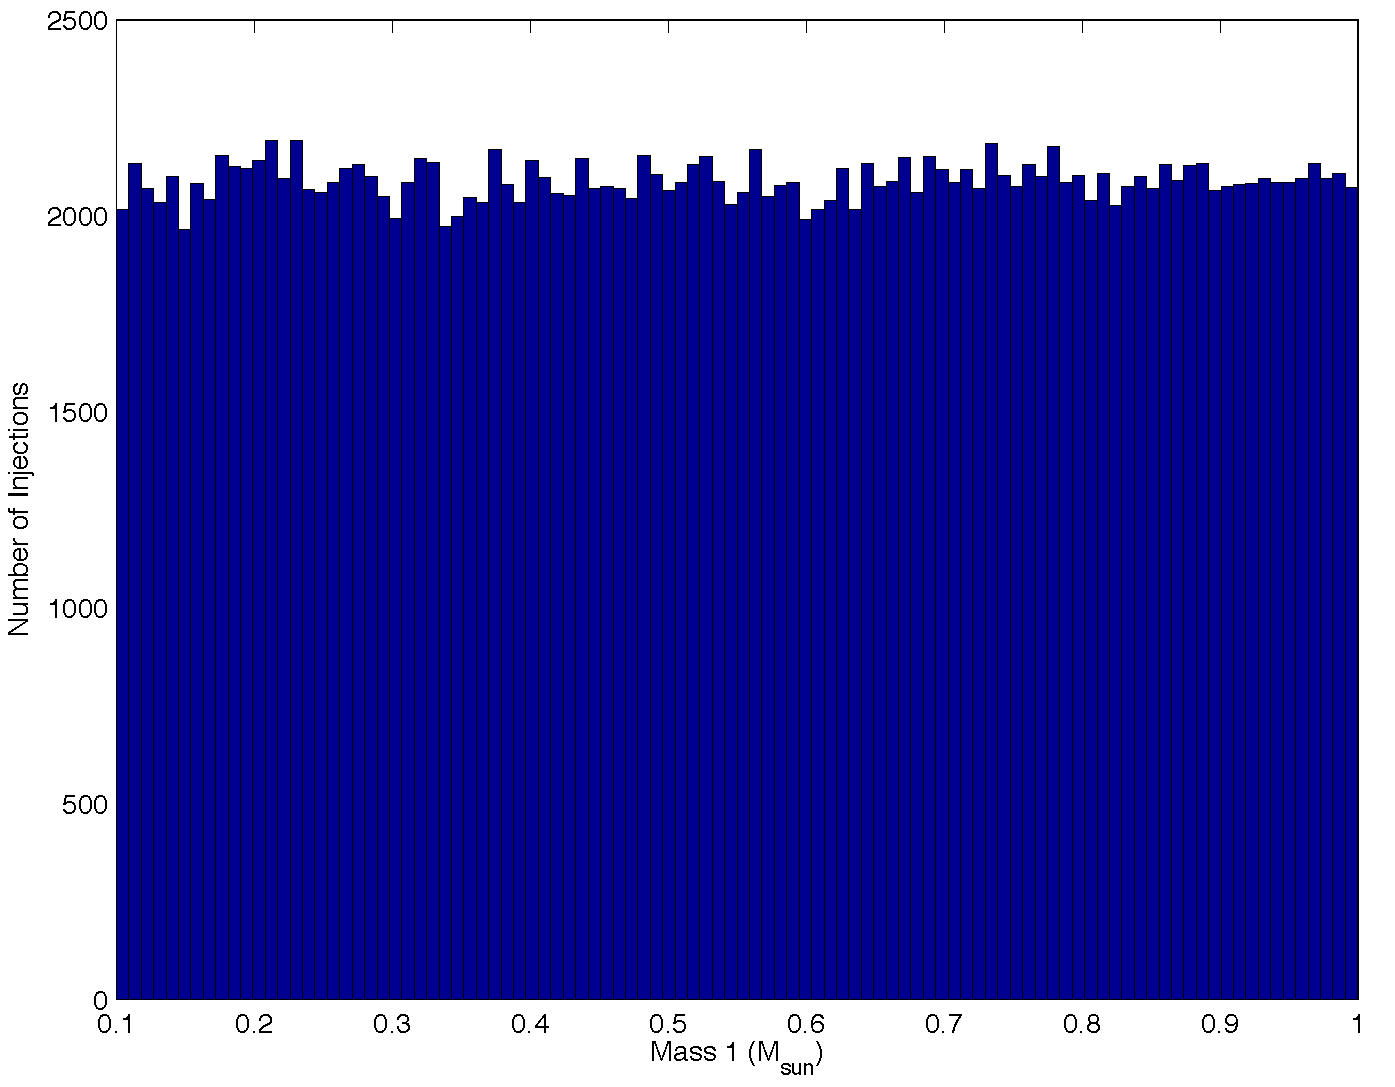
\includegraphics[width=\linewidth]{figures/macho/m1_hist}
\end{center}
\caption{\label{f:m1_hist}%
The BBHMACHO population Monte Carlo code is used to simulate a distribution of
$209048$ coalescing binaries. The distribution of the first component mass,
$m_1$ is then histogramed to confirm that it is uniformly distributed over the
expected range, as shown. Similar tests are performed for the second mass
parameter, $m_2$, the galactocentic longitude, $\theta$, the inclination
angle, $\iota$, the polarization angle, $\psi$, and the coalescence phase,
$\phi_c$.
}
\end{figure}

\begin{figure}[p]
\begin{center}
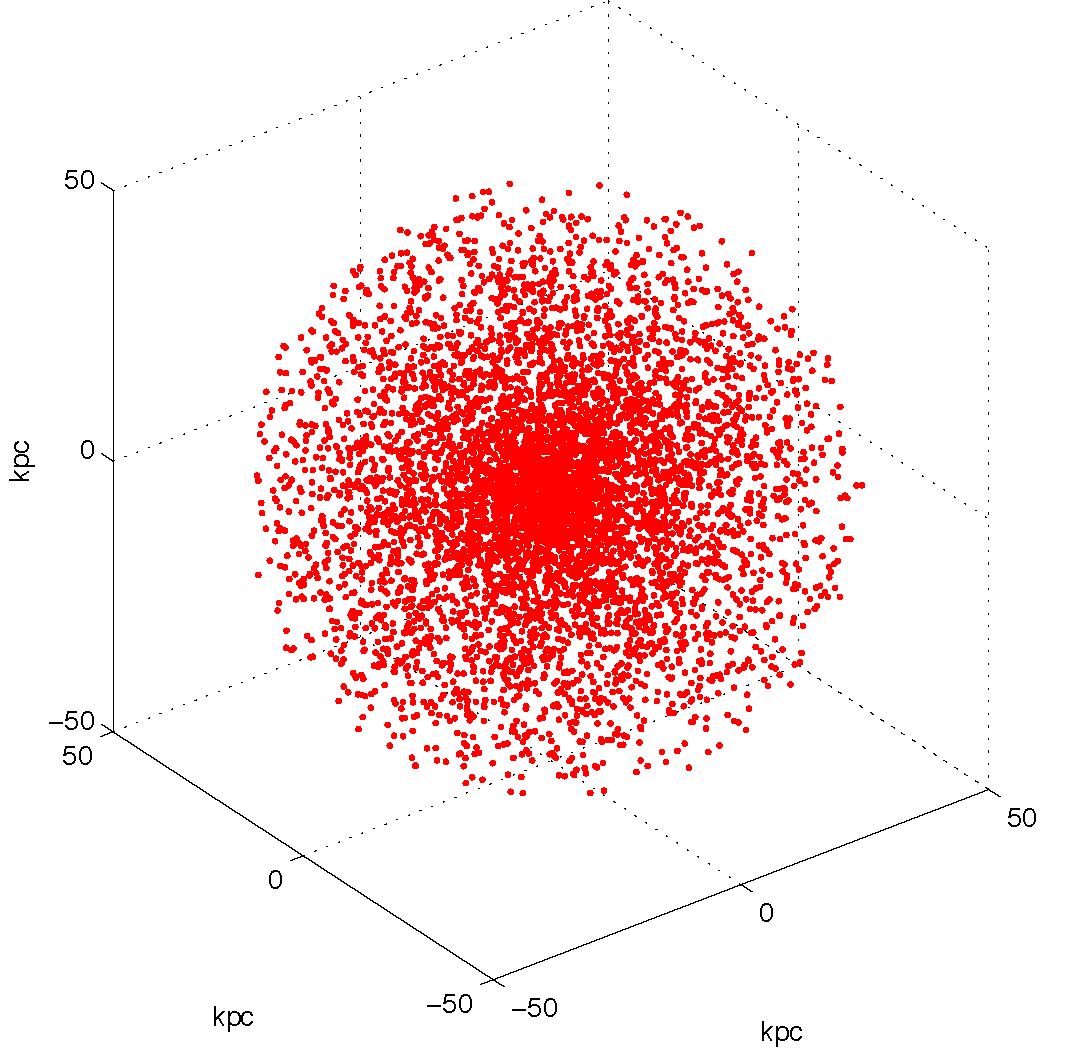
\includegraphics[width=\linewidth]{figures/macho/spherical_cartesian}
\end{center}
\caption{\label{f:spherical_cartesian}%
The spatial distribution of $5000$ simulated BBHMACHO binaries in a spherical,
$q=0$, Galactic halo of size $R_\mathrm{max} = 50\,\mathrm{kpc}$ with a core
radius $a = 8.5\,\mathrm{kpc}$ shown in galactocentric coordinates. Each point
in the figure corresponds to a simulated BBHMACHO injection.
}
\end{figure}

\begin{figure}[p]
\begin{center}
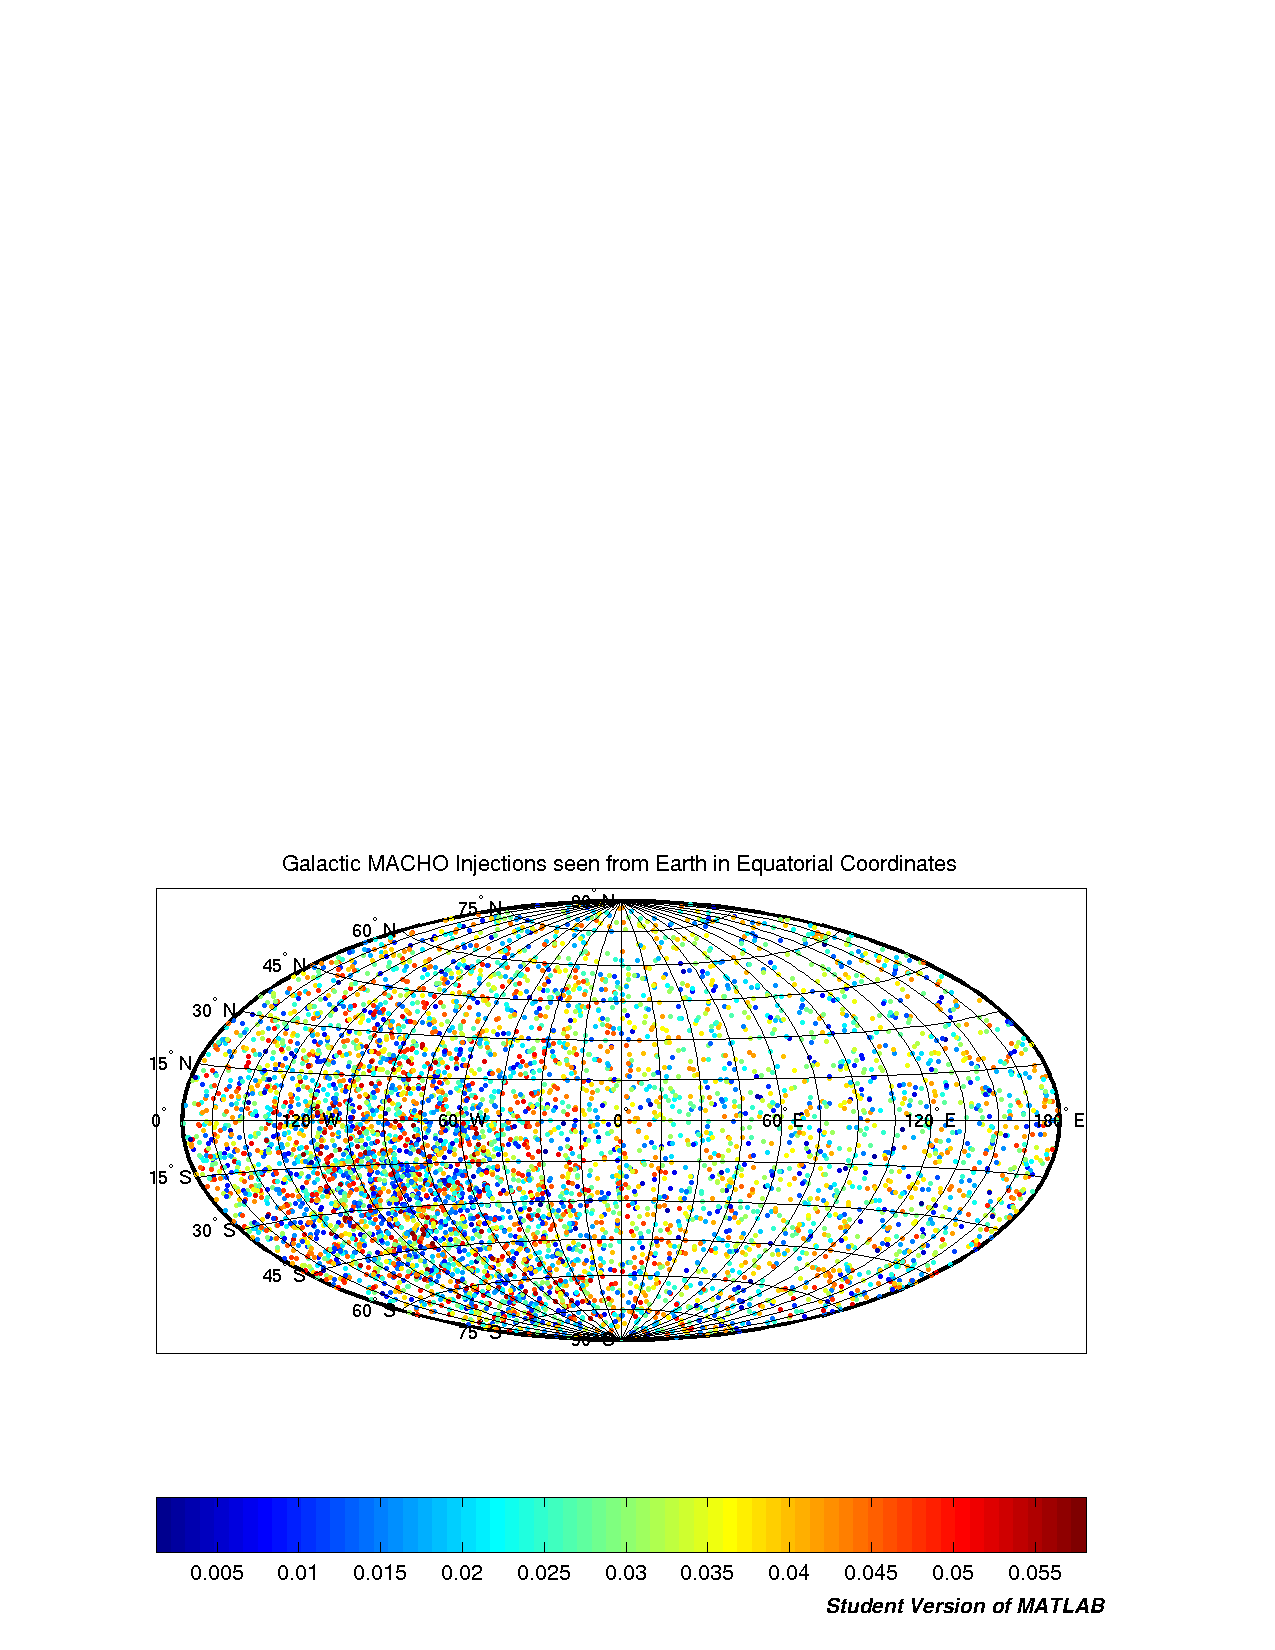
\includegraphics[width=\linewidth]{figures/macho/spherical_equatorial}
\end{center}
\caption{\label{f:spherical_equatorial}%
The spatial distribution of $5000$ simulated BBHMACHO binaries in a spherical,
$q=0$, Galactic halo of size $R_\mathrm{max} = 50\,\mathrm{kpc}$ with a core
radius $a = 8.5\,\mathrm{kpc}$ shown in equatorial coordinates. Each point
in the figure corresponds to a simulated BBHMACHO injection. The color of the
point shows the distance from the center of the earth to the binary. Note the
dense clump of binaries in the southern hemisphere, towards the center of the
galaxy.
}
\end{figure}




